\documentclass[journal]{IEEEtran}
\onecolumn
\linespread{2}

\usepackage{graphicx}
\usepackage{booktabs}
\usepackage{amsmath}
\usepackage{amssymb}
\usepackage{array}
\usepackage{url}
\usepackage[hidelinks]{hyperref}
\usepackage{xcolor}

\renewcommand{\ttdefault}{cmtt}

\hypersetup{
  pdftitle={Few-Shot Image Classification with Foundation Models: A Comparative Study of ViT and DINOv3 Adaptation Strategies},
  pdfauthor={Nitish Kumar Gundapu},
  pdfsubject={CS 6350 TPA-17 Term Project Report}
}

\hyphenation{op-tical net-works semi-conduc-tor pa-ram-e-ter}

\begin{document}

\title{Few-Shot Image Classification with Foundation Models: A Comparative Study of ViT and DINOv3 Adaptation Strategies}

\author{Nitish~Kumar~Gundapu% <-this % stops a space
}

\markboth{CS 6350 Term Project Assignment Report}%
{Gundapu: Few-Shot Classification with Foundation Models}

\IEEEspecialpapernotice{TPA-17}

\maketitle

\begin{abstract}
Foundation models provide strong visual representations, but adapting them to a
new domain with only a handful of labels remains an open practical question.
This report studies five adaptation strategies for two vision foundation
models: full fine-tuning, linear probing, LoRA, BitFit, and a training-free
nearest-class-mean (NCM) prototype classifier. The comparison uses
Google ViT-B/16 and DINOv3 ViT-B/16 on Flowers102 and CIFAR-100 with ten
labeled images per class. Both datasets are evaluated on their official held-out
test splits, and every run records top-1/top-5 accuracy, macro F1, trainable
parameters, wall-clock training time, and peak GPU memory. On CIFAR-100, frozen
DINOv3 features are the strongest choice: NCM reaches 81.64\% top-1 and linear
probing reaches 81.44\% while updating only 0.09\% of the parameters, whereas
full fine-tuning reaches 58.02\%. On Flowers102 the representation is already
saturated: ViT reaches 98.49--99.15\% across methods, and DINOv3 linear probing
and NCM both reach about 99.7\%. The results show that, in the low-data regime,
the choice of frozen representation and a well-regularized head can matter more
than the number of trainable parameters. We also quantify the sensitivity of
DINOv3 full fine-tuning to the learning rate and provide representation,
attention, and confusion-matrix diagnostics from the developed pipelines.
\end{abstract}

\section{Introduction}
\IEEEPARstart{F}{oundation} models such as ViT, CLIP, and DINO have changed the
way visual recognition systems are built. Instead of training a task-specific
network from scratch, a pretrained backbone is adapted to a downstream dataset.
The adaptation is easy when the target domain is large, but many realistic
applications provide only a few labeled examples per class. Medical imaging,
remote sensing, manufacturing inspection, and fine-grained biological
classification all face this low-data regime. The central question of this
project is therefore not whether a foundation model can classify images, but
which adaptation strategy gives the best accuracy and resource trade-off when
only ten labeled images per class are available.

The project brief asks for a reproducible pipeline that compares zero-shot or
training-free evaluation, linear probing, full fine-tuning, and parameter-efficient
adapter methods on foundation models. We implemented two pipelines with a common
experimental protocol:
\begin{itemize}
  \item a ViT pipeline based on Hugging Face \texttt{transformers}, using
        \texttt{google/vit-base-patch16-224};
  \item a DINOv3 pipeline based on \texttt{timm}, using the ungated
        \texttt{vit\_base\_patch16\_dinov3.lvd1689m} checkpoint.
\end{itemize}
Both pipelines support five strategies: full fine-tuning, linear probing (LP),
LoRA, BitFit, and nearest-class-mean (NCM). We evaluate them on Flowers102 and
CIFAR-100 under a fixed ten-shot protocol and report accuracy, macro F1,
parameter count, training time, and peak GPU memory.

The main findings are as follows. First, on CIFAR-100, frozen DINOv3 features
are substantially better than updating the backbone: NCM (81.64\%) and linear
probing (81.44\%) outperform full fine-tuning (58.02\%) and LoRA (59.77\%).
Second, Flowers102 is saturated by both pretrained representations, so most
methods fall within a narrow band near 99\%, and the interesting axis becomes
efficiency rather than raw accuracy. Third, DINOv3 full fine-tuning is highly
learning-rate sensitive: the shared $10^{-4}$ rate collapses to 13.90\% top-1,
while $2\times10^{-5}$ recovers 58.02\%. Fourth, the training-free NCM baseline
is the most efficient method by a wide margin, requiring no optimizer and
roughly 7--15 seconds of feature extraction.

The remainder of the report is organized as follows. Section~II reviews related
work. Section~III describes the datasets, models, adaptation strategies, and
evaluation protocol. Section~IV presents the results and diagnostics.
Section~V discusses implications and limitations, and Section~VI concludes.

\section{Related Work}
\subsection{Vision Foundation Models}
The Vision Transformer (ViT) applies a Transformer encoder to a sequence of
image patches and showed that large-scale pretraining can match or exceed
convolutional networks \cite{dosovitskiy2021vit}. DINOv2 learned general-purpose
visual features with self-supervised distillation and demonstrated strong
transfer without task-specific labels \cite{oquab2024dinov2}. DINOv3 extends
this line with larger-scale self-supervised training and improved dense and
global features \cite{simeoni2025dinov3}. CLIP took a different route, aligning
images and text through contrastive pretraining and enabling text-prompt
zero-shot classification \cite{radford2021clip}. The present study uses ViT and
DINOv3 because both are widely available as image-only backbones. Neither has a
text encoder, so true text-prompt zero-shot classification is not available in
this setup; NCM is used as the training-free alternative.

\subsection{Efficient Adaptation}
Full fine-tuning updates every backbone parameter, which is expensive and prone
to overfitting when labels are scarce. Linear probing freezes the backbone and
trains only a classifier, and it is often a surprisingly strong baseline for
frozen foundation features. Adapter methods insert small trainable modules into
a frozen network \cite{houlsby2019adapters}. LoRA decomposes weight updates into
low-rank matrices and has become a standard parameter-efficient method for
Transformers \cite{hu2022lora}. BitFit updates only the bias terms of the
network \cite{zaken2022bitfit}. Our implementation follows these definitions:
LoRA is applied to attention projections, and BitFit updates all bias terms plus
the classification head.

\subsection{Few-Shot Classification}
Prototypical networks classify a query by its distance to class means computed
from a small support set \cite{snell2017prototypical}. Nearest-class-mean
classifiers are an early and effective instance of this idea for large-scale
image classification \cite{mensink2012ncm}. In this report the NCM baseline
$L_2$-normalizes frozen CLS features, averages the ten examples of each class,
and assigns the class with the highest cosine similarity. It requires no
gradient updates and no classifier training, which makes it a clean lower bound
for the value of adaptation.

\subsection{Datasets and Diagnostics}
Flowers102 is a fine-grained 102-class flower dataset introduced for
large-scale flower classification \cite{nilsback2008flowers}. CIFAR-100 is a
standard 100-class image classification benchmark \cite{krizhevsky2009cifar}.
For visualization we use t-SNE to project validation embeddings
\cite{vandermaaten2008tsne} and Grad-CAM to inspect the spatial evidence used by
the transformer \cite{selvaraju2017gradcam}. The implementation relies on
PyTorch Lightning \cite{falcon2019lightning}, Hugging Face Transformers
\cite{wolf2020transformers}, timm \cite{wightman2019timm}, and PEFT
\cite{mangrulkar2022peft}; classification metrics and plots use scikit-learn
and Matplotlib \cite{pedregosa2011sklearn}.

\section{Methodology}
\subsection{Pipeline Overview}
Figure~\ref{fig:pipeline} summarizes the experimental pipeline. A dataset is
converted into a deterministic few-shot training split and held-out validation
and test splits. The chosen backbone is loaded with pretrained weights, the
adaptation strategy determines which parameters are trainable, and the resulting
model is evaluated on accuracy, F1, parameter count, time, and memory. Each run
also writes prediction arrays and diagnostic figures that feed the comparison
report.

\begin{figure}[t]
  \centering
  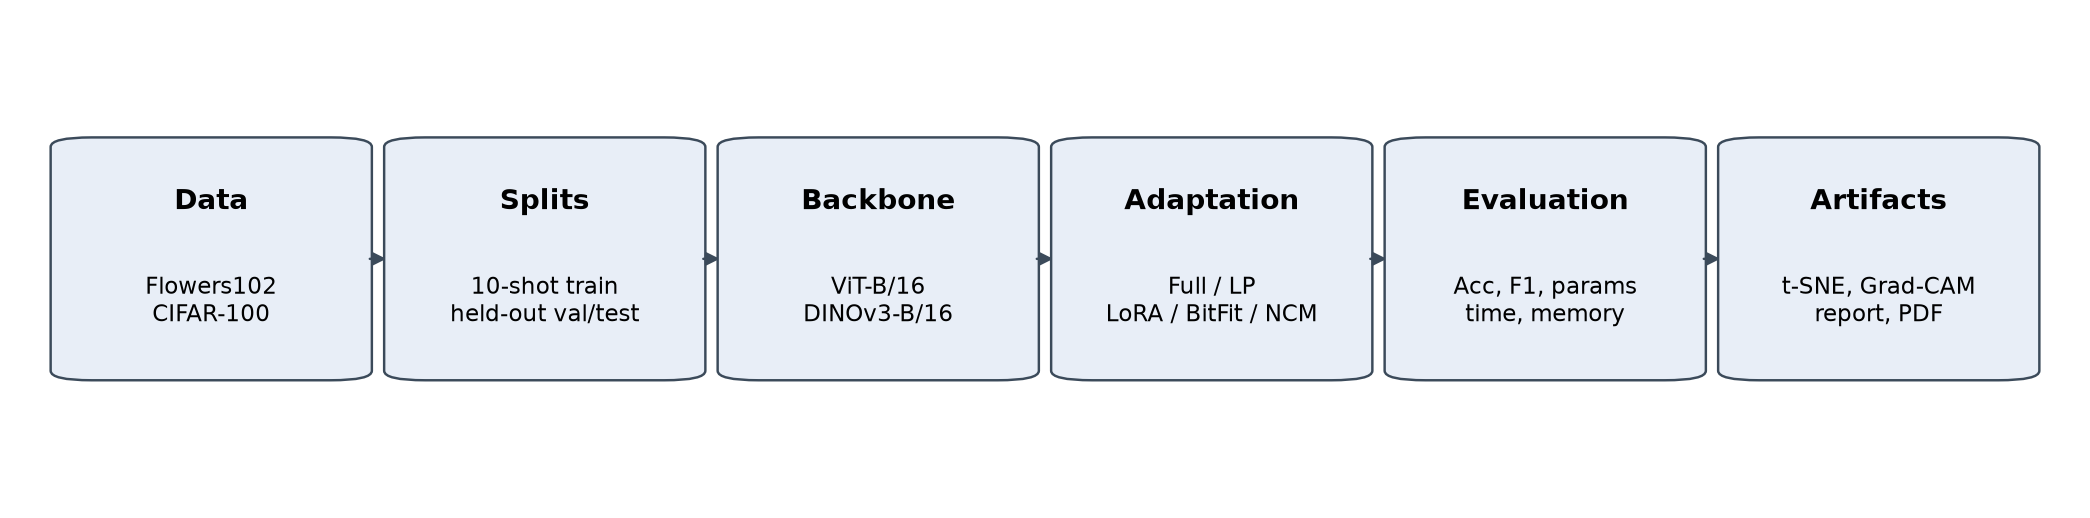
\includegraphics[width=\linewidth]{figures/fig_pipeline.png}
  \caption{End-to-end pipeline used for both foundation models. The same data
  splits, metrics, and artifact writers are shared by the ViT and DINOv3
  implementations.}
  \label{fig:pipeline}
\end{figure}

\subsection{Datasets and Few-Shot Splits}
\textbf{Flowers102.} The dataset contains 8{,}189 images from 102 flower
classes. The official training split has ten images per class, so the ten-shot
setting uses the full training split (1{,}020 images). Validation and test use
the official splits of 1{,}020 and 6{,}149 images. Images are RGB and have
variable resolution.

\textbf{CIFAR-100.} The dataset contains 50{,}000 training images and 10{,}000
test images from 100 classes. Because the official training set does not define
a validation split, we hold out ten images per class (1{,}000 images) for model
selection and sample ten additional images per class from the remaining pool for
training. The official 10{,}000-image test split is used unchanged. The split is
deterministic given the seed and was verified to have no train/validation
overlap.

Table~\ref{tab:training} lists the training settings. The ViT Flowers102
experiments use the original 30-epoch schedule of the ViT pipeline. The CIFAR-100
experiments and the DINOv3 Flowers102 experiments use a shorter 10-epoch
schedule to keep the full comparison tractable. All runs use seed 42, a
cosine-annealed AdamW optimizer, weight decay 0.05, and early stopping on
validation loss with patience 3 (10 for the original ViT Flowers102 runs).
Learning rates are reported per method because the optimal rate differs sharply
between full fine-tuning and a linear head.

\begin{table}[t]
  \caption{Training settings. LR values are listed in the order full / LP /
  LoRA / BitFit.}
  \label{tab:training}
  \centering
  \small
  \setlength{\tabcolsep}{5pt}
  \begin{tabular}{lcccc}
    \toprule
    Setting & Flowers ViT & Flowers DINOv3 & CIFAR ViT & CIFAR DINOv3 \\
    \midrule
    Epochs              & 30 & 10 & 10 & 10 \\
    Batch size          & 16 & 32 & 32 & 32 \\
    Shots per class     & 10 & 10 & 10 & 10 \\
    Full LR             & $10^{-4}$ & $2\times10^{-5}$ & $10^{-4}$ & $2\times10^{-5}$ \\
    LP LR               & $10^{-4}$ & $10^{-3}$ & $10^{-3}$ & $10^{-3}$ \\
    LoRA / BitFit LR    & $10^{-4}$ & $10^{-4}$ & $10^{-4}$ & $10^{-4}$ \\
    Weight decay        & 0.05 & 0.05 & 0.05 & 0.05 \\
    \bottomrule
  \end{tabular}
\end{table}

\subsection{Models and Preprocessing}
\textbf{ViT-B/16.} We use \texttt{google/vit-base-patch16-224}, a ViT-Base
model with patch size $16\times16$ and 224$\times$224 input resolution. The
classification head is replaced with a 102-way or 100-way linear layer as
appropriate. Images are processed with the model's Hugging Face image processor.

\textbf{DINOv3-B/16.} We use the timm checkpoint
\texttt{vit\_base\_patch16\_dinov3.lvd1689m}. The checkpoint is loaded through
the ungated timm mirror because the corresponding Hugging Face repository is
gated. DINOv3 uses 256$\times$256 input resolution, bicubic interpolation, and
ImageNet normalization, as specified by its pretrained configuration. The
backbone exposes a CLS token plus storage tokens; we use the CLS token as the
global image representation.

For training, both pipelines use random-resized cropping with scale
$(0.65,1.0)$, random horizontal flipping, and normalization. DINOv3 preprocessing
is resolved from the pretrained timm configuration. The DINOv3 augmentation
deliberately omits color jitter to keep the comparison closer to a standard
linear-probe protocol.

\subsection{Adaptation Strategies}
Let $f_\theta$ be the frozen backbone and $h_\phi$ the linear classification
head. The five strategies are:

\begin{enumerate}
  \item \textbf{Full fine-tuning.} All backbone and head parameters are
  trainable. This is the most expressive and most expensive option.
  \item \textbf{Linear probing (LP).} The backbone is frozen and only $h_\phi$
  is trained. For ViT-B/16 this is 76{,}900 parameters on CIFAR-100 and 78{,}438
  on Flowers102; the difference is the number of classes.
  \item \textbf{LoRA.} Low-rank updates are added to attention projections. We
  use rank $r=16$, $\alpha=32$, and dropout 0.1. For ViT the target modules are
  \texttt{q\_proj} and \texttt{v\_proj}; for timm DINOv3 they are
  \texttt{attn.qkv} and \texttt{attn.proj}. The head remains fully trainable.
  \item \textbf{BitFit.} All bias terms in the backbone and the full head are
  trainable; all weight matrices stay frozen.
  \item \textbf{Nearest-class-mean (NCM).} No parameters are trained. For each
  class $c$, the prototype is
  \begin{equation}
    \mu_c = \frac{1}{|\mathcal{S}_c|}\sum_{i\in\mathcal{S}_c}
    \frac{f_\theta(x_i)}{\lVert f_\theta(x_i)\rVert_2},
  \end{equation}
  and a test image is assigned to
  $\arg\max_c \cos(f_\theta(x),\mu_c)$. This is the training-free baseline.
\end{enumerate}

\subsection{Evaluation Protocol}
For every run we report top-1 accuracy, top-5 accuracy, macro-averaged F1,
weighted F1, the number of trainable parameters, the trainable fraction, the
wall-clock training time, and peak GPU memory. Metrics are computed on the
official test split after model selection on the validation split. We also store
per-class F1, confusion matrices, validation CLS embeddings, and Grad-CAM
visualizations.

The main hardware is an NVIDIA RTX PRO 4000 Blackwell GPU with 24~GB of memory.
The software stack uses PyTorch 2.14, PyTorch Lightning, timm 1.0.30,
Transformers 5.19, and PEFT 0.21. The complete pipeline is configured with a
single command-line interface and writes a structured results directory.

\subsection{Algorithmic Summary}
The training and evaluation procedure can be summarized as follows.
\begin{enumerate}
  \item Build the deterministic training, validation, and test splits from the
  selected dataset.
  \item Load the pretrained backbone and replace the classifier with a linear
  head for the target number of classes.
  \item Apply the selected adaptation strategy: unfreeze all parameters, the
  head only, LoRA adapters, or bias terms. For NCM, skip optimization.
  \item Optimize trainable parameters with cross-entropy loss and AdamW for the
  configured number of epochs, selecting the checkpoint with the lowest
  validation loss.
  \item Extract logits and CLS embeddings for validation and test, compute
  metrics, and write predictions, confusion matrices, t-SNE plots, and Grad-CAM
  grids.
  \item Aggregate all runs into a comparison table and trade-off plots.
\end{enumerate}

\subsection{Reproducibility}
All experiments are driven by the command-line interfaces in
\texttt{src/vit} and \texttt{src/dino\_v3}. The main CIFAR-100 sweeps are
reproduced with
\begin{verbatim}
python -m src.vit.main sweep --dataset cifar100 \
  --methods full lp lora bitfit ncm --shots-per-class 10 \
  --epochs 10 --patience 3 --batch-size 32

python -m src.dino_v3.main sweep --dataset cifar100 \
  --methods full lp lora bitfit ncm --shots-per-class 10 \
  --epochs 10 --patience 3 --batch-size 32
\end{verbatim}
The Flowers102 experiments use \texttt{--dataset flowers102}. Per-run outputs
are written to \texttt{results/<dataset>/<method>/seed\_42/} for ViT and
\texttt{results/dino\_v3/<dataset>/<method>/seed\_42/} for DINOv3, and the
aggregated tables and plots are written to the corresponding
\texttt{analysis/} directory. Each run records the configuration, metrics,
checkpoint path, predictions, per-class F1, confusion matrix, t-SNE plot, and
Grad-CAM grid.

\section{Results and Discussion}
\subsection{Overall Comparison}
Tables~\ref{tab:cifar} and~\ref{tab:flowers} report the complete results.
Figure~\ref{fig:cifarbars} visualizes the CIFAR-100 top-1 and macro-F1 scores,
and Figure~\ref{fig:flowersbars} shows the same comparison on Flowers102.

\begin{table}[t]
  \caption{CIFAR-100 results, ten shots per class, seed 42. All methods use the
  learning rates in Table~\ref{tab:training}.}
  \label{tab:cifar}
  \centering
  \footnotesize
  \setlength{\tabcolsep}{3.5pt}
  \resizebox{\linewidth}{!}{%
  \begin{tabular}{llccccccc}
    \toprule
    Model & Method & Top-1 & Top-5 & Macro F1 & Trainable & \% Train. & Time (s) & GPU (MB) \\
    \midrule
    ViT-B/16 & Full      & 0.7834 & 0.9501 & 0.7831 & 85{,}875{,}556 & 100.00 & 155.5 & 4987 \\
             & LP        & 0.7783 & 0.9415 & 0.7796 & 76{,}900       & 0.09   & 88.5  & 633  \\
             & LoRA      & 0.6328 & 0.8862 & 0.6206 & 666{,}724      & 0.77   & 122.1 & 3344 \\
             & BitFit    & 0.5936 & 0.8528 & 0.5806 & 179{,}812      & 0.21   & 118.7 & 2802 \\
             & NCM       & 0.7761 & 0.9370 & 0.7785 & 0              & 0.00   & 13.4  & 618  \\
    \midrule
    DINOv3-B/16 & Full   & 0.5802 & 0.8538 & 0.5604 & 85{,}718{,}116 & 100.00 & 201.8 & 7362 \\
                & LP     & 0.8144 & 0.9627 & 0.8150 & 76{,}900       & 0.09   & 113.1 & 710  \\
                & LoRA   & 0.5977 & 0.8563 & 0.5771 & 961{,}636      & 1.11   & 170.9 & 4908 \\
                & BitFit & 0.5106 & 0.7735 & 0.4954 & 152{,}164      & 0.18   & 159.1 & 4171 \\
                & NCM    & 0.8164 & 0.9624 & 0.8173 & 0              & 0.00   & 14.9  & 702  \\
    \bottomrule
  \end{tabular}}
\end{table}

\begin{table}[t]
  \caption{Flowers102 results, ten shots per class, seed 42. ViT uses 30 epochs;
  DINOv3 uses 10 epochs.}
  \label{tab:flowers}
  \centering
  \footnotesize
  \setlength{\tabcolsep}{3.5pt}
  \resizebox{\linewidth}{!}{%
  \begin{tabular}{llccccccc}
    \toprule
    Model & Method & Top-1 & Top-5 & Macro F1 & Trainable & \% Train. & Time (s) & GPU (MB) \\
    \midrule
    ViT-B/16 & Full      & 0.9849 & 0.9980 & 0.9854 & 85{,}877{,}094 & 100.00 & 435.1 & 3182 \\
             & LP        & 0.9867 & 0.9974 & 0.9850 & 78{,}438       & 0.09   & 217.3 & 512  \\
             & LoRA      & 0.9912 & 0.9977 & 0.9899 & 668{,}262      & 0.77   & 320.7 & 1870 \\
             & BitFit    & 0.9915 & 0.9972 & 0.9907 & 181{,}350      & 0.21   & 311.1 & 1596 \\
             & NCM       & 0.9859 & 0.9971 & 0.9833 & 0              & 0.00   & 6.2   & 489  \\
    \midrule
    DINOv3-B/16 & Full   & 0.9647 & 0.9940 & 0.9636 & 85{,}719{,}654 & 100.00 & 191.2 & 7362 \\
                & LP     & 0.9971 & 0.9982 & 0.9965 & 78{,}438       & 0.09   & 101.3 & 710  \\
                & LoRA   & 0.9787 & 0.9971 & 0.9762 & 963{,}174      & 1.11   & 158.6 & 4908 \\
                & BitFit & 0.9639 & 0.9956 & 0.9584 & 153{,}702      & 0.18   & 147.7 & 4171 \\
                & NCM    & 0.9969 & 0.9984 & 0.9963 & 0              & 0.00   & 7.6   & 702  \\
    \bottomrule
  \end{tabular}}
\end{table}

\begin{figure}[t]
  \centering
  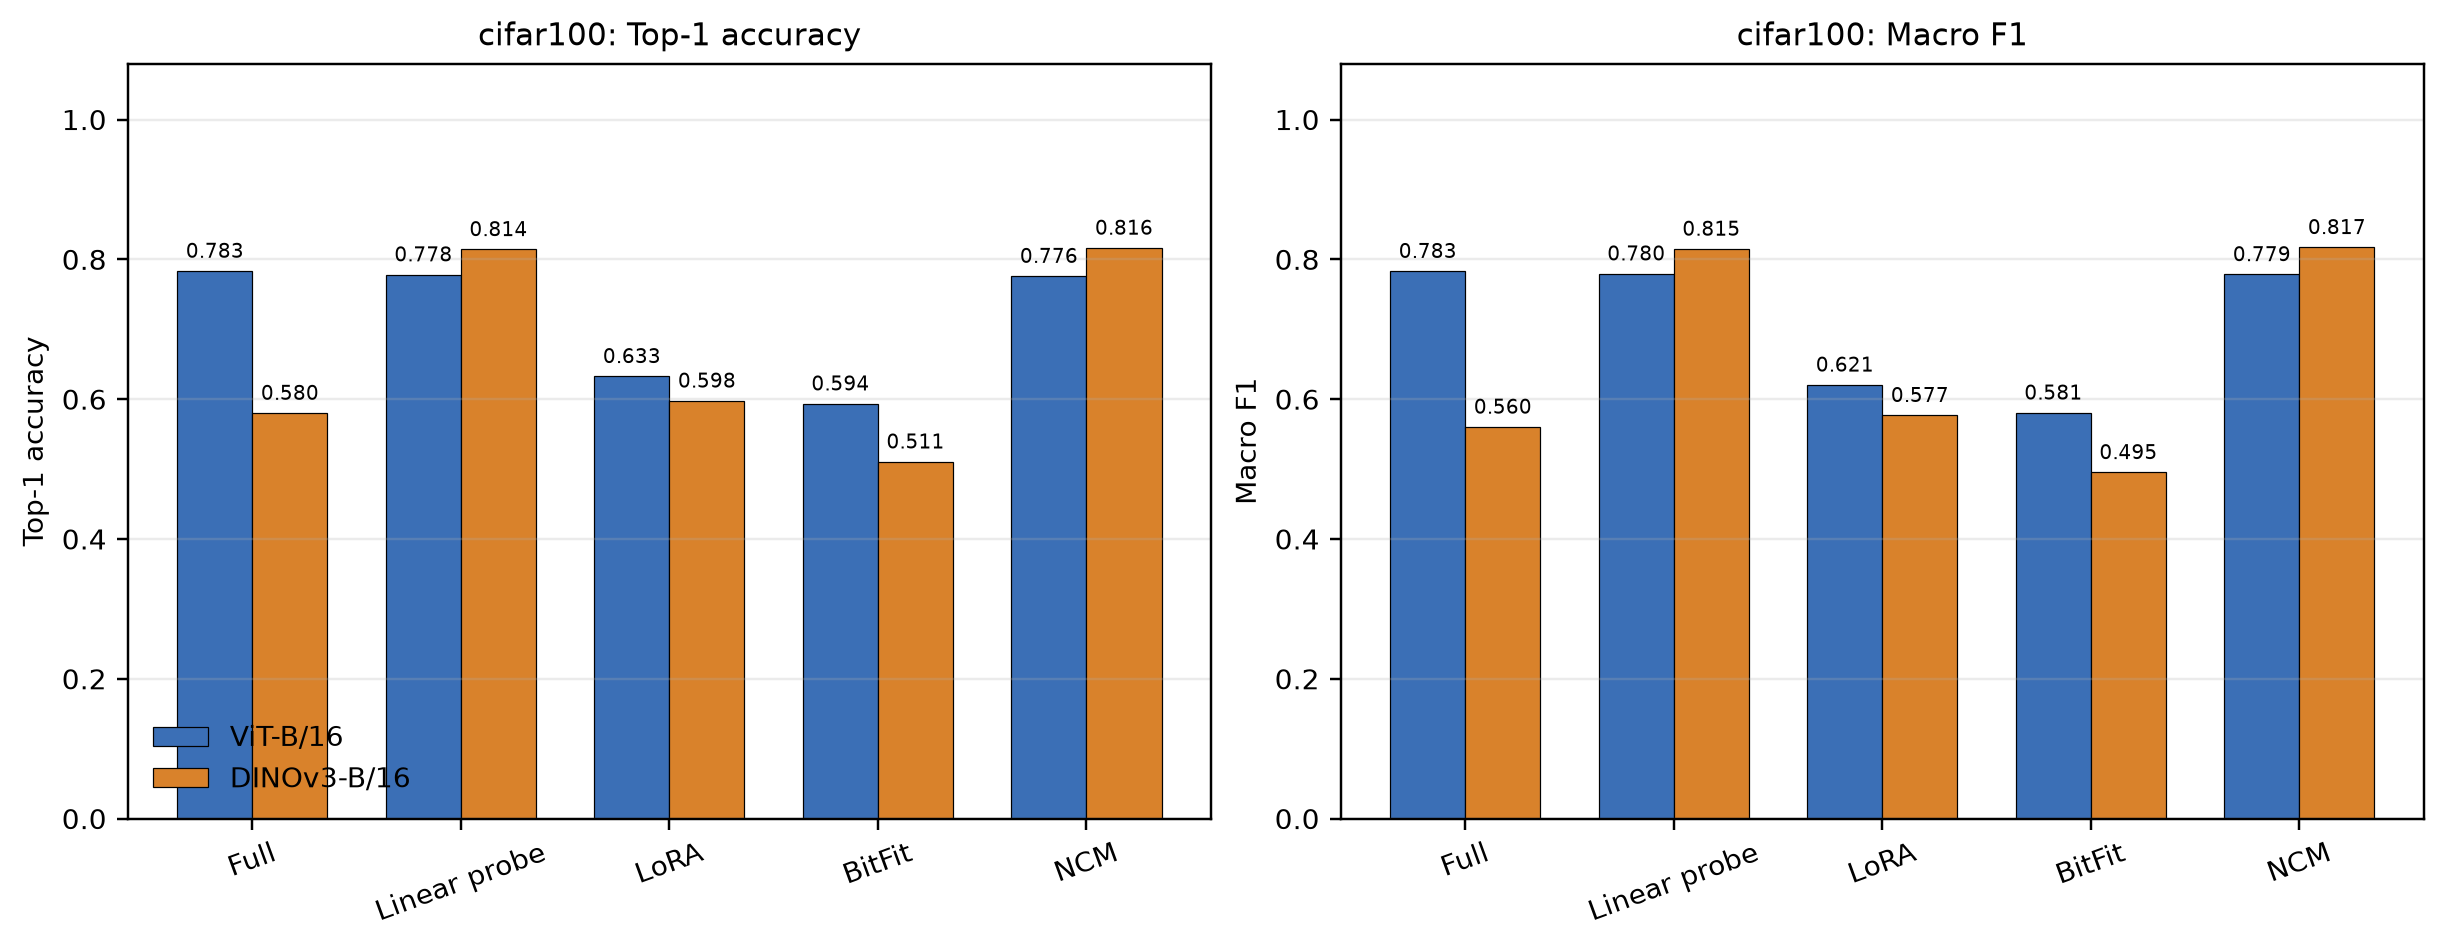
\includegraphics[width=\linewidth]{figures/fig_cifar_bars.png}
  \caption{CIFAR-100 comparison of ViT-B/16 and DINOv3-B/16 for the five
  adaptation strategies. Left: top-1 accuracy. Right: macro F1. NCM is
  training-free and has zero trainable parameters.}
  \label{fig:cifarbars}
\end{figure}

\begin{figure}[t]
  \centering
  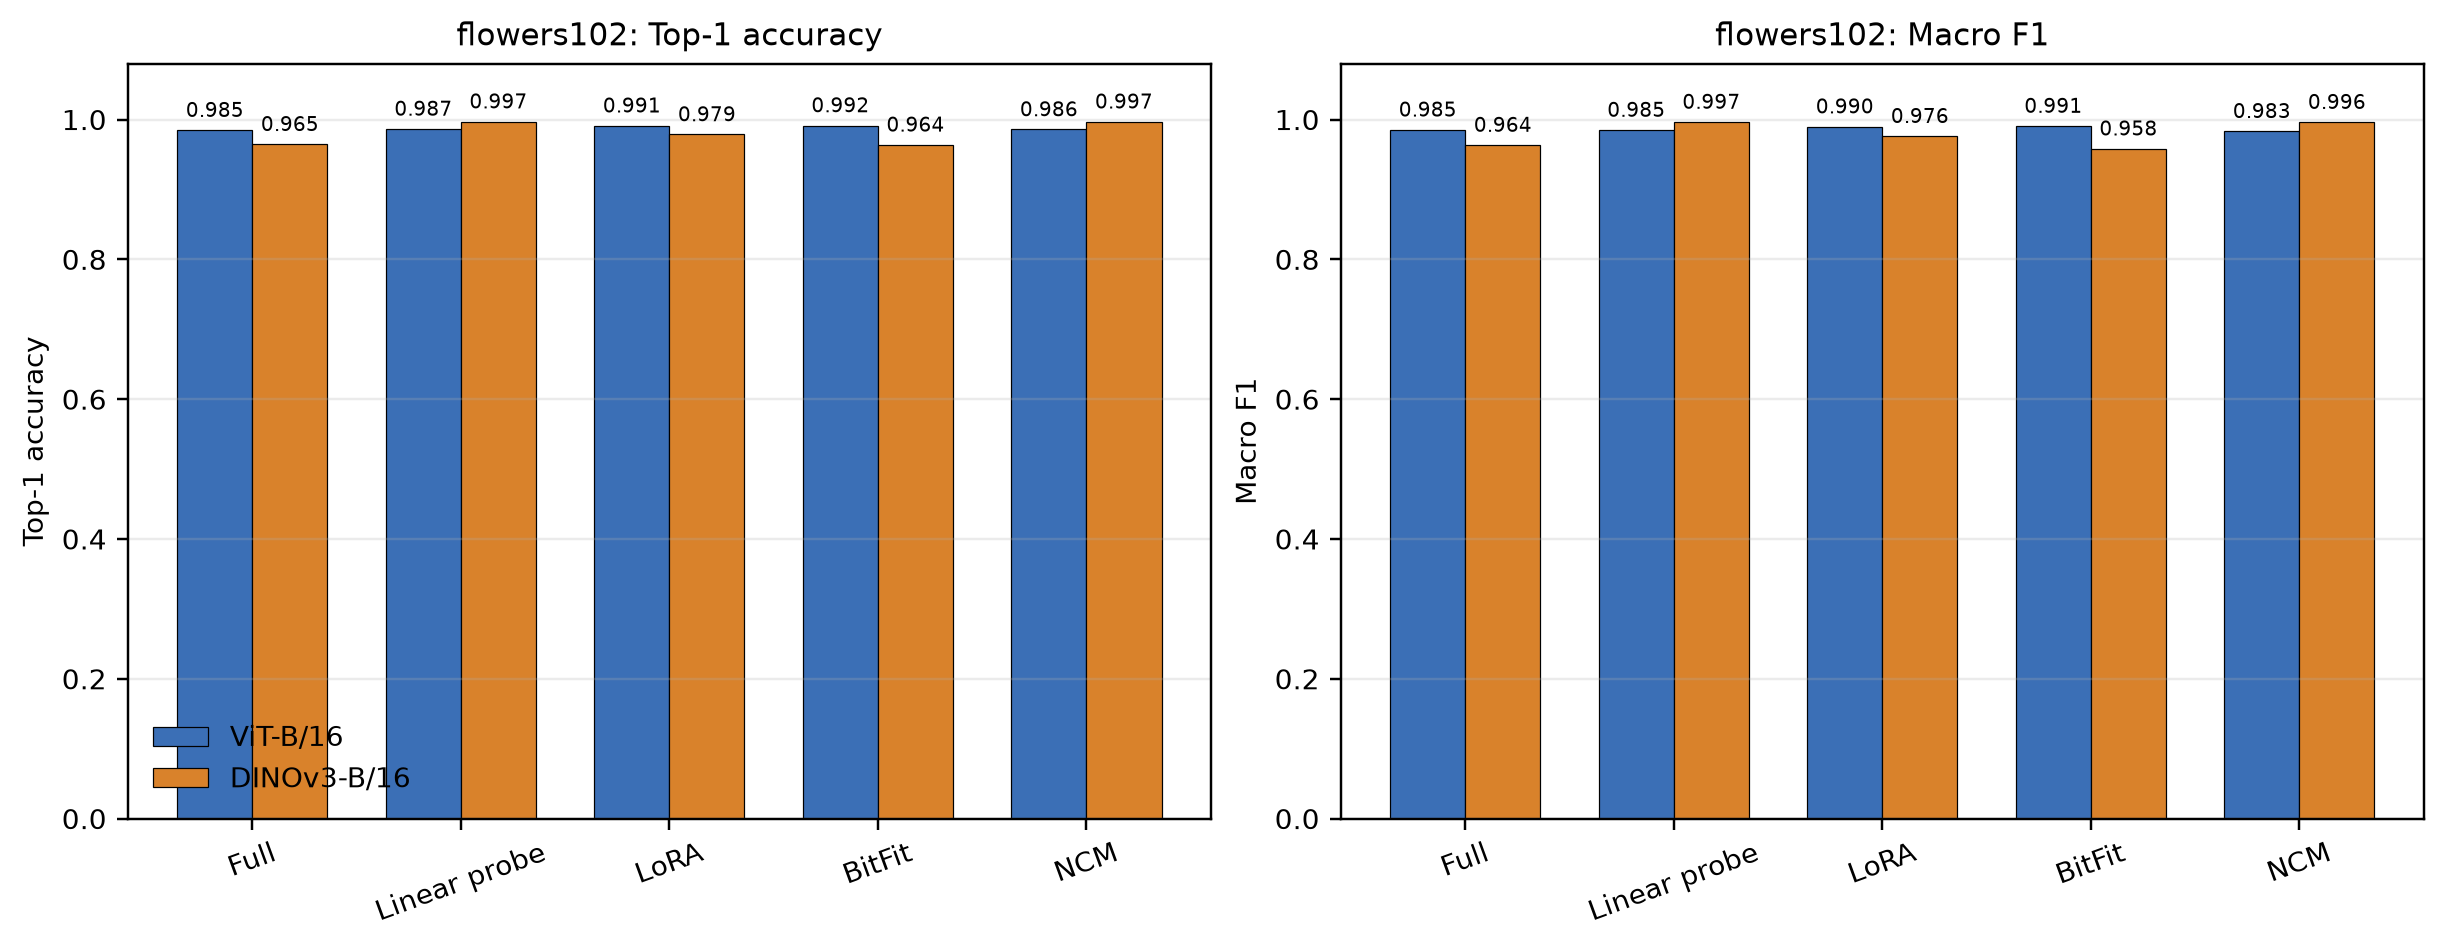
\includegraphics[width=\linewidth]{figures/fig_flowers_bars.png}
  \caption{Flowers102 comparison. The ViT runs use 30 epochs; the DINOv3 runs
  use 10 epochs. The dataset is saturated by both pretrained
  representations, so most methods lie within a narrow accuracy band.}
  \label{fig:flowersbars}
\end{figure}

\subsection{Observations}
\textbf{CIFAR-100 favors frozen DINOv3 features.} The best CIFAR-100 result is
DINOv3 NCM at 81.64\% top-1 and 81.73\% macro F1, followed closely by DINOv3
linear probing at 81.44\% and 81.50\%. Linear probing trains only 76{,}900
parameters, which is 0.09\% of the 85.7M-parameter backbone. Full fine-tuning
and LoRA reach only 58.02\% and 59.77\%, respectively. With ten images per
class, updating the backbone appears to overfit or to move the representation
away from the pretrained solution. The NCM result shows that the frozen DINOv3
CLS features are already highly discriminative for the 100 CIFAR-100 classes.

\textbf{ViT is more balanced on CIFAR-100.} ViT full fine-tuning reaches 78.34\%,
linear probing 77.83\%, and NCM 77.61\%, all within 0.8 points. LoRA (63.28\%)
and BitFit (59.36\%) are clearly worse under the same ten-epoch schedule. The
ViT linear probe required a higher learning rate ($10^{-3}$) than the backbone
updates; at $10^{-4}$ it reached only 50.78\%, which shows that the same
optimizer setting is not equally suitable for a randomly initialized head and
a pretrained backbone.

\textbf{Flowers102 is saturated.} On Flowers102 every method reaches at least
96.39\% top-1, and most are above 98.5\%. ViT BitFit is the best ViT method
(99.15\%), while DINOv3 linear probing and NCM reach 99.71\% and 99.69\%,
respectively. The narrow spread indicates that the Flowers102 representation is
already close to linearly separable, so the choice of adaptation method matters
much less than on CIFAR-100. DINOv3 full fine-tuning and BitFit are the lowest
DINOv3 results at 96.47\% and 96.39\%, respectively, but both remain far above
the CIFAR-100 full fine-tuning result.

\textbf{Efficiency.} Figure~\ref{fig:efficiency} plots accuracy against trainable
parameters and training time on CIFAR-100. NCM has zero trainable parameters and
takes 13.4--14.9 seconds, while linear probing takes 88.5--113.1 seconds.
Full fine-tuning takes 155.5--201.8 seconds and uses 5.0--7.4~GB of GPU memory.
The NCM and LP points dominate the accuracy-per-parameter frontier on this
dataset. The full fine-tuning point is not on the frontier even though it uses
three orders of magnitude more parameters.

\begin{figure}[t]
  \centering
  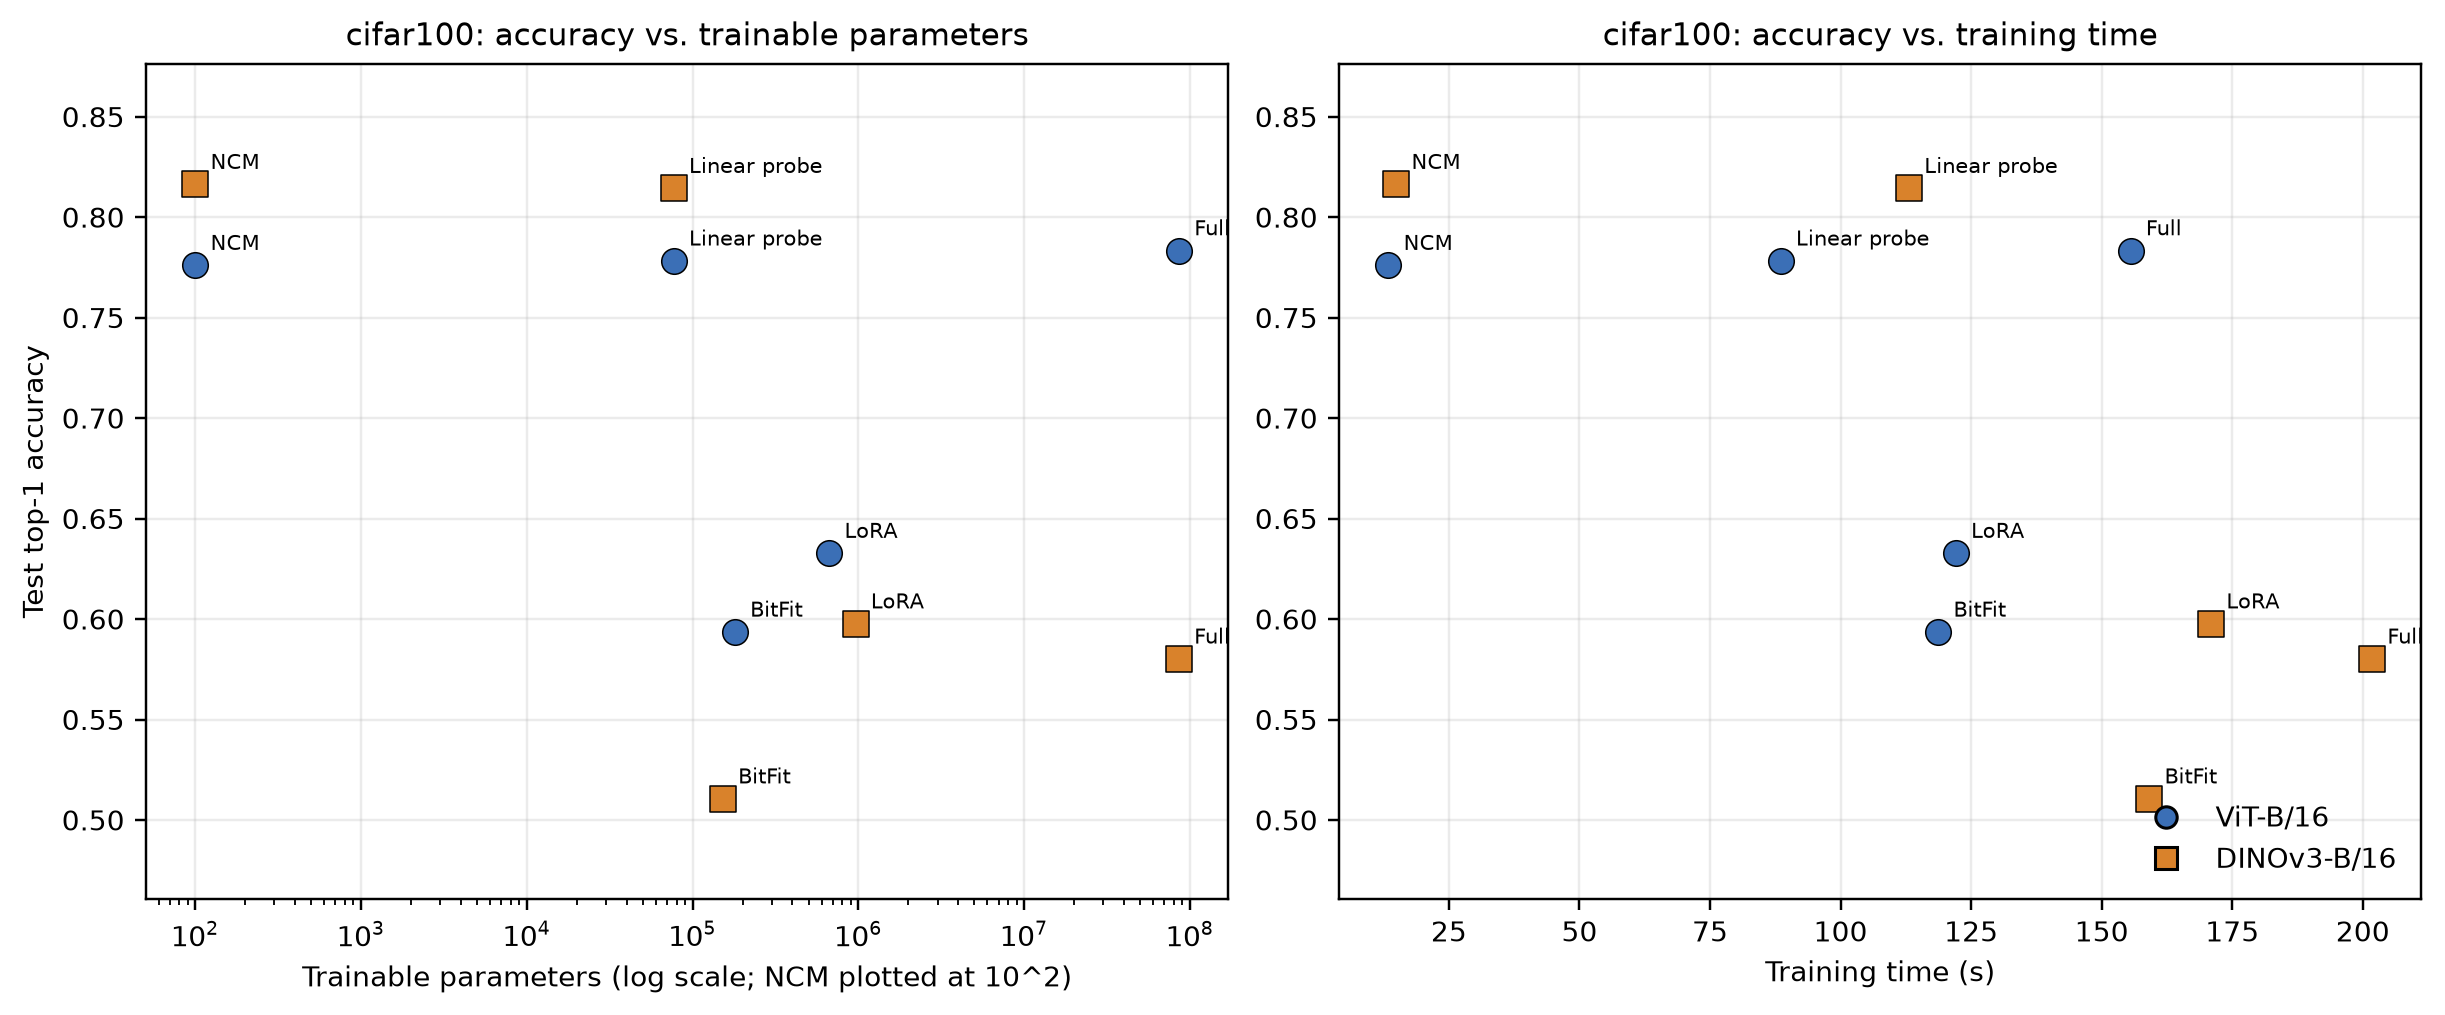
\includegraphics[width=\linewidth]{figures/fig_cifar_efficiency.png}
  \caption{CIFAR-100 accuracy versus trainable parameters (left, log scale) and
  training time (right). NCM has zero trainable parameters and is placed at
  $10^2$ on the logarithmic axis for visibility.}
  \label{fig:efficiency}
\end{figure}

\textbf{Per-class behavior.} Figure~\ref{fig:perclass} shows the distribution of
per-class F1 over the 100 CIFAR-100 classes. DINOv3 LP and NCM have high medians
and relatively compact lower tails, whereas DINOv3 full fine-tuning and BitFit
have much wider distributions, with many classes below 0.5 F1. ViT full and LP
also have high medians, but LoRA and BitFit show a long lower tail. This
indicates that the aggregate accuracy is not hiding a small number of
catastrophic classes in the best methods.

\begin{figure}[t]
  \centering
  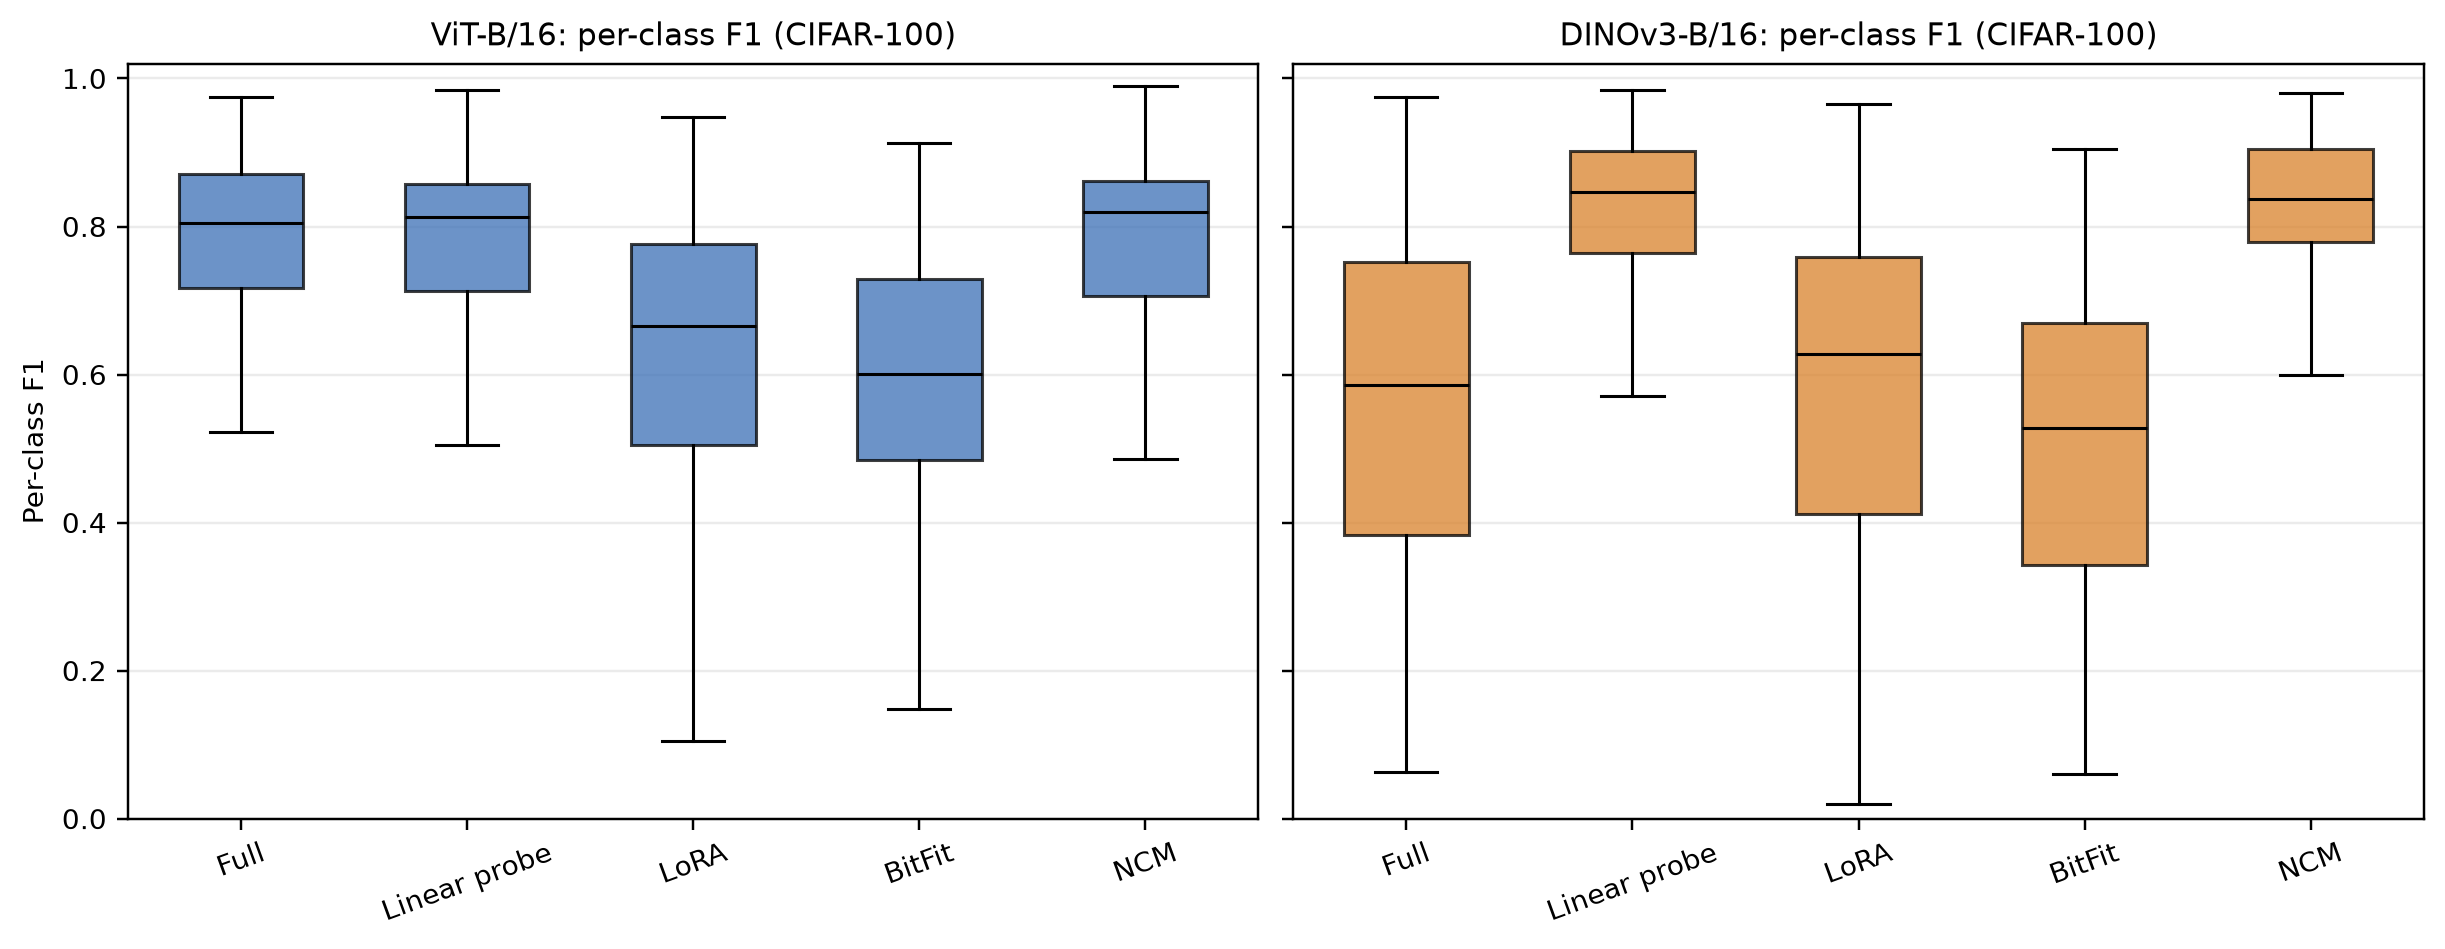
\includegraphics[width=\linewidth]{figures/fig_per_class_f1.png}
  \caption{Distribution of per-class F1 over the 100 CIFAR-100 classes. Boxes
  show the interquartile range and the median; whiskers extend to the
  non-outlier range.}
  \label{fig:perclass}
\end{figure}

\textbf{Learning-rate sensitivity.} DINOv3 full fine-tuning is markedly more
sensitive to the learning rate than the other methods. With the shared
$10^{-4}$ rate it reaches only 13.90\% top-1 on CIFAR-100; with
$2\times10^{-5}$ it reaches 58.02\%. DINOv3 linear probing shows the opposite
trend: $10^{-4}$ gives 45.47\%, while $10^{-3}$ gives 81.44\%. This is a
practical warning for cross-model comparisons: a single global learning rate can
make a strong method look weak. The reported tables use the per-method values in
Table~\ref{tab:training}, and we record the learning rate in each run's metrics
file.

\subsection{Representation and Attention Diagnostics}
Figure~\ref{fig:tsne} compares t-SNE projections of validation CLS embeddings
for ViT full fine-tuning and DINOv3 linear probing on CIFAR-100. Both models
form visible class clusters, but the DINOv3 projection contains many compact,
well-separated groups despite never updating the backbone. This is consistent
with the strong NCM and LP results: the frozen representation already organizes
the 100 classes into linearly separable regions, and the linear head mostly
learns the class boundaries.

\begin{figure}[t]
  \centering
  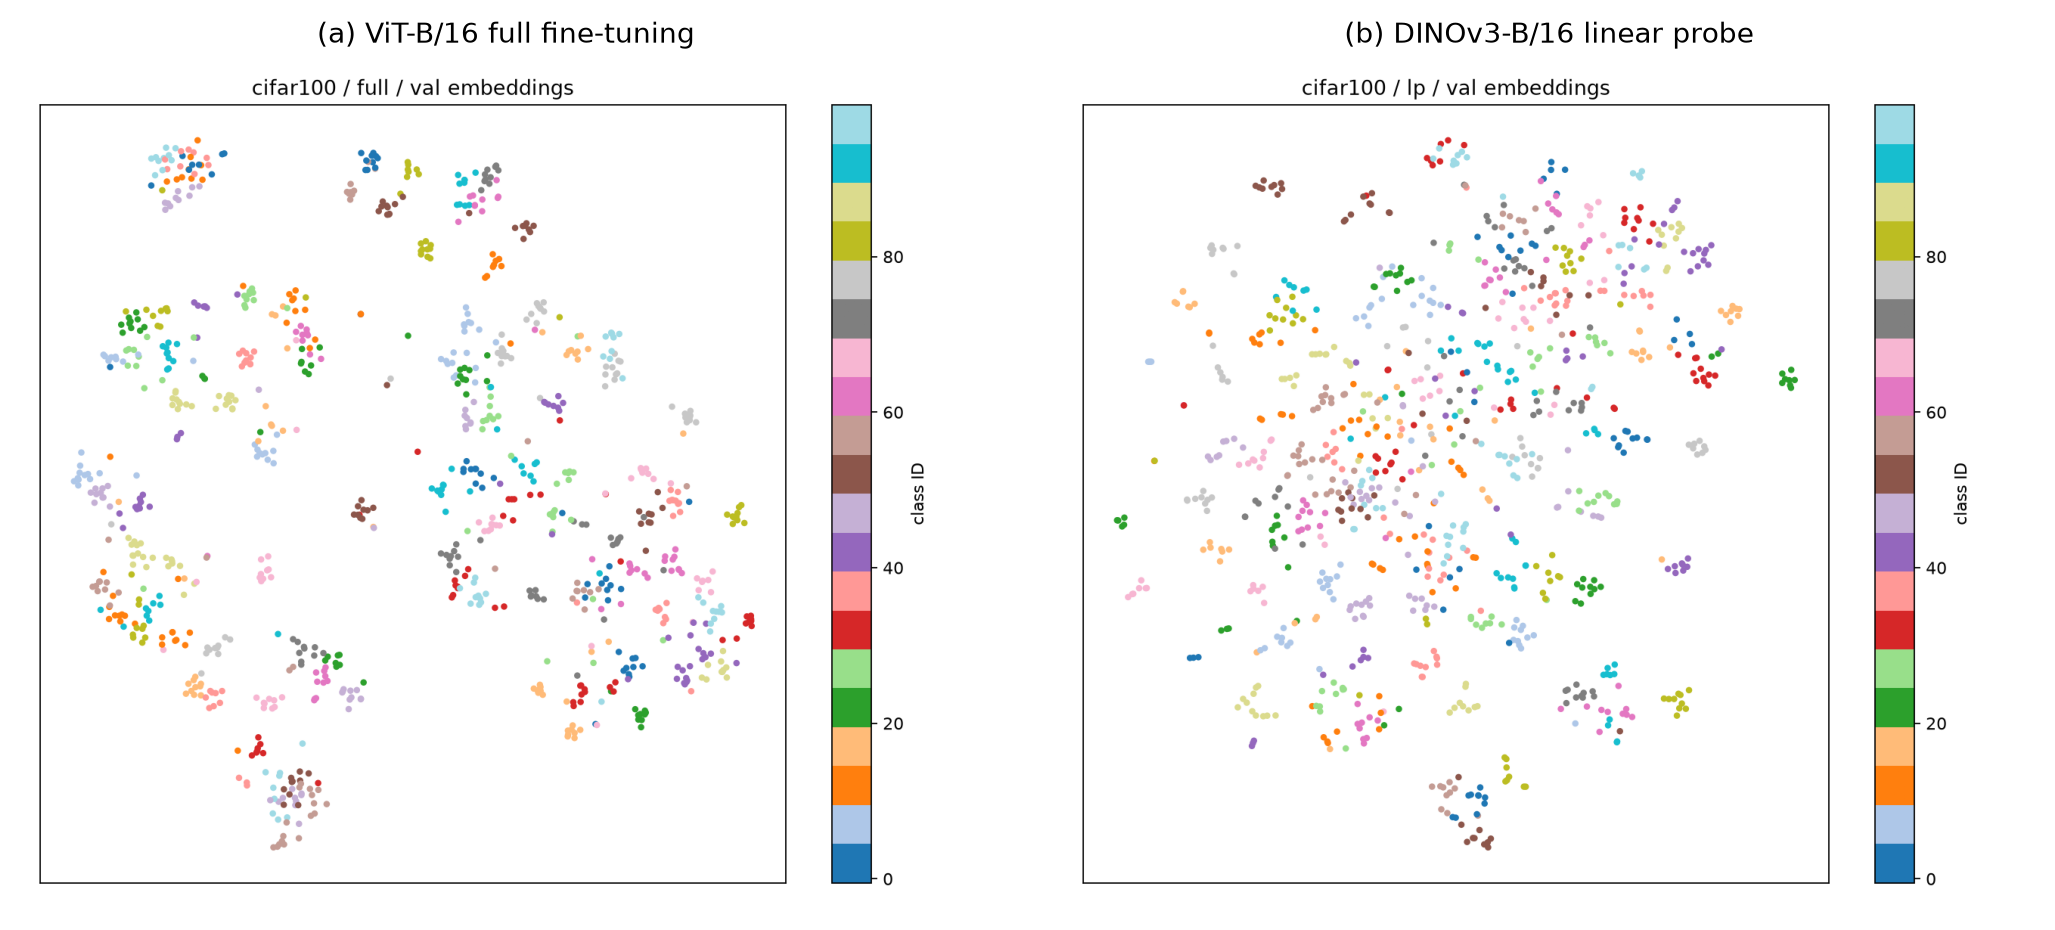
\includegraphics[width=\linewidth]{figures/fig_tsne_compare.png}
  \caption{t-SNE projections of CIFAR-100 validation CLS embeddings.
  (a) ViT-B/16 full fine-tuning. (b) DINOv3-B/16 linear probing. Colors denote
  class IDs. The DINOv3 features form compact, separated clusters without
  backbone updates.}
  \label{fig:tsne}
\end{figure}

Figure~\ref{fig:gradcam} shows Grad-CAM maps from the last transformer block.
The ViT examples highlight object parts and local regions, while the DINOv3
examples tend to place attention on the object itself and on its immediate
context. The maps are not perfect: one DINOv3 sample with true class 42 is
predicted as class 31, and the attention is spread across the animal and the
background. Nevertheless, the successful examples show that both backbones
attend to semantically relevant regions rather than to arbitrary image
corners.

\begin{figure}[t]
  \centering
  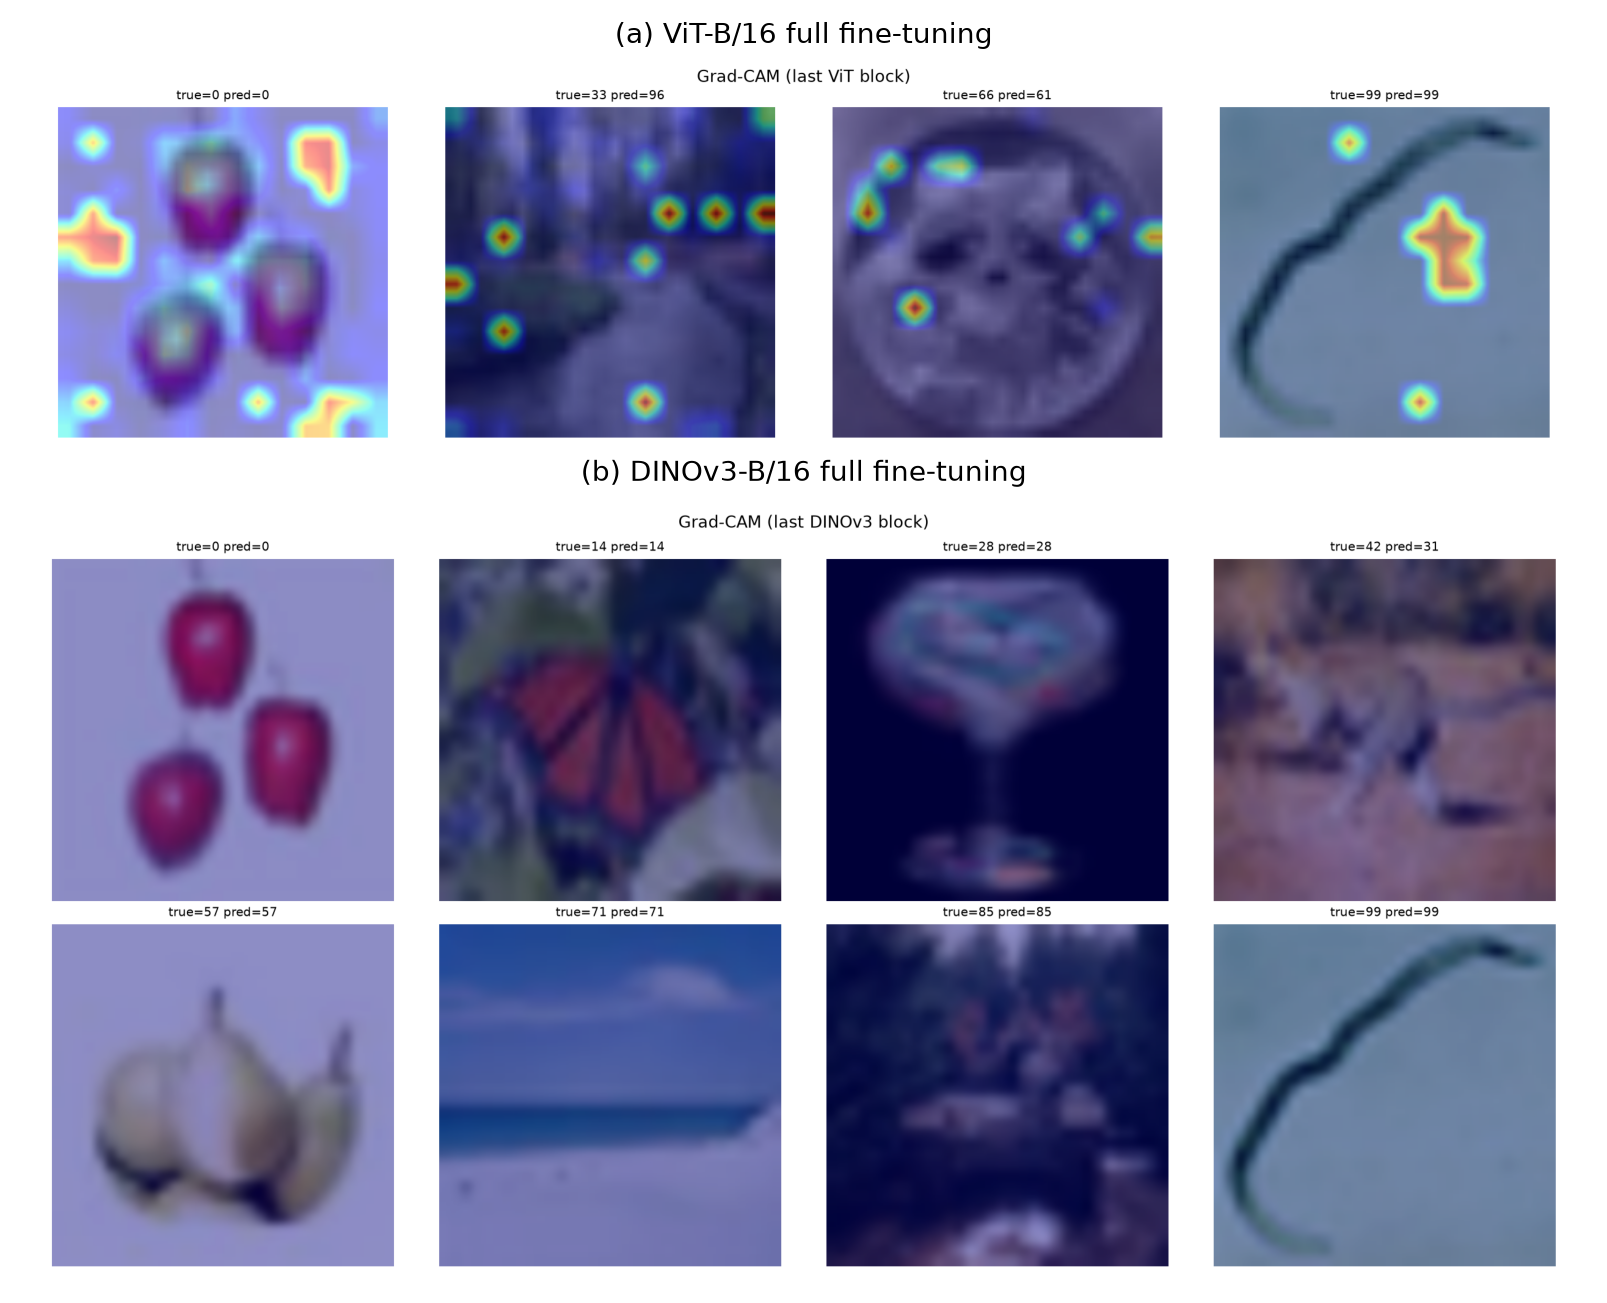
\includegraphics[width=\linewidth]{figures/fig_gradcam_compare.png}
  \caption{Grad-CAM visualizations from the last transformer block on
  CIFAR-100 validation images. (a) ViT-B/16 full fine-tuning. (b) DINOv3-B/16
  full fine-tuning. Each panel is labeled with the true and predicted class.}
  \label{fig:gradcam}
\end{figure}

Figure~\ref{fig:confusion} compares row-normalized confusion matrices for the
two strongest CIFAR-100 configurations. The diagonals are dominant in both
cases, but the DINOv3 LP matrix has fewer off-diagonal cells with visible mass.
The remaining errors are concentrated among visually similar classes, which is
expected for 32$\times$32 images upscaled to the backbone input resolution.

\begin{figure}[t]
  \centering
  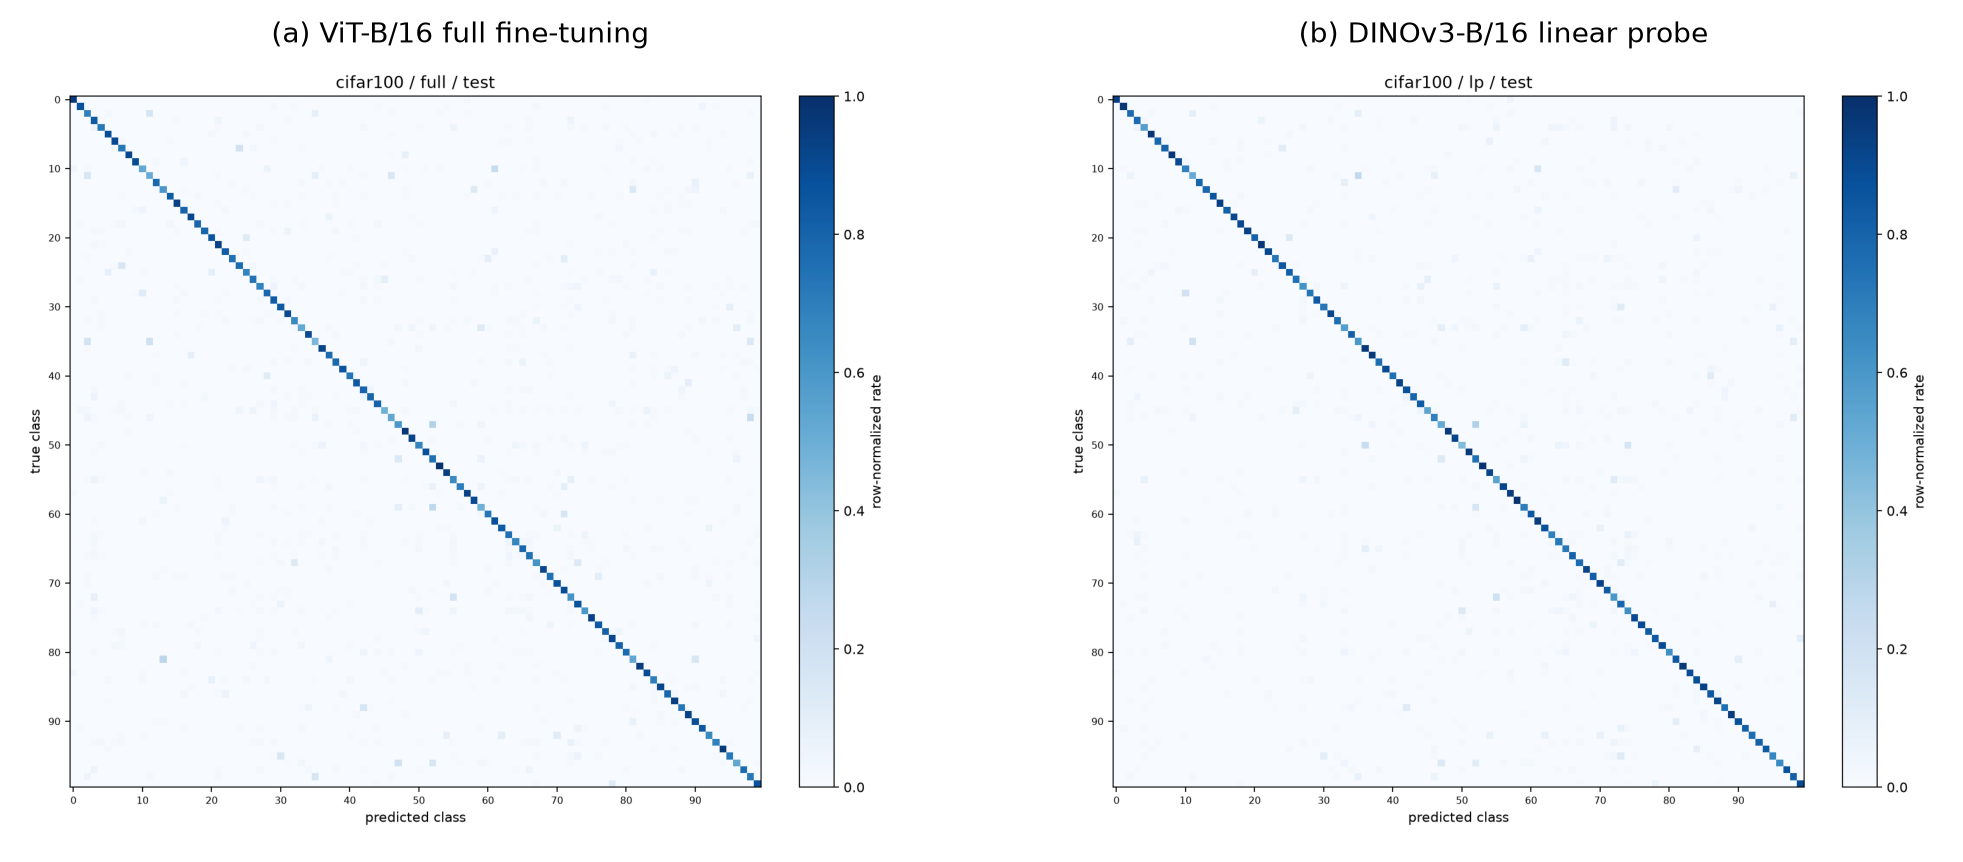
\includegraphics[width=\linewidth]{figures/fig_confusion_compare.png}
  \caption{Row-normalized CIFAR-100 test confusion matrices. (a) ViT-B/16 full
  fine-tuning. (b) DINOv3-B/16 linear probing.}
  \label{fig:confusion}
\end{figure}

\subsection{Discussion}
The results lead to a clear practical recommendation for ten-shot
classification. If a strong self-supervised backbone such as DINOv3 is
available, start with NCM or linear probing. Both are cheap, stable, and in our
CIFAR-100 experiments more accurate than full fine-tuning or LoRA. NCM is
especially attractive when there is no budget for optimization: it requires one
forward pass over the support set, no gradients, and no hyperparameter search
beyond the feature normalization and similarity scale.

The Flowers102 results show the opposite regime. When the target domain is close
to the pretraining distribution and the features are already highly separable,
ViT LoRA (99.12\%) and BitFit (99.15\%) slightly exceed ViT linear probing
(98.67\%), while DINOv3 linear probing remains the best DINOv3 method (99.71\%).
The differences are small, however, and the training cost is much higher. This
suggests that adaptation effort should be allocated based on the difficulty of
the target dataset rather than applied uniformly.

The ViT and DINOv3 results also illustrate the importance of matching the
optimizer to the adaptation strategy. A linear head trained from scratch needs a
larger learning rate than a pretrained backbone that is being gently updated.
DINOv3 full fine-tuning needs a smaller rate than ViT full fine-tuning on the
same data. Reporting a single global learning rate without this tuning would
lead to misleading conclusions about which architecture or method is better.

\textbf{Limitations.} The study uses a single seed and a single short schedule
for most runs, so the absolute numbers should be treated as a controlled
snapshot rather than a fully converged benchmark. CIFAR-100 images are
32$\times$32 and are upscaled to 224 or 256 pixels, which limits fine-grained
accuracy. The ViT Flowers102 runs use 30 epochs while the remaining runs use 10,
so the Flowers102 cross-model comparison is not perfectly matched. We did not
evaluate CLIP or a text-prompt zero-shot baseline, because the two selected
backbones do not contain a text encoder. Finally, the NCM scale and the LoRA
rank were fixed rather than tuned per dataset.

\textbf{Future work.} Natural extensions are to repeat the comparison across
multiple seeds, to match the training schedule across models and datasets, to
add CLIP-style zero-shot evaluation, and to test adapters and prefix tuning.
It would also be useful to evaluate on a genuinely shifted domain, such as
medical or remote-sensing images, where the gap between frozen features and
full fine-tuning may be larger. Calibration and selective prediction are
additional directions, since the confusion matrices show that the remaining
errors are concentrated in a subset of visually similar classes.

\section{Conclusion}
We developed reproducible ViT and DINOv3 pipelines and compared full
fine-tuning, linear probing, LoRA, BitFit, and NCM under a ten-shot protocol on
Flowers102 and CIFAR-100. On CIFAR-100, frozen DINOv3 features are the best
choice: NCM reaches 81.64\% and linear probing 81.44\%, while full fine-tuning
and LoRA remain below 60\%. On Flowers102 the representation is saturated and
all methods are close to 99\%. NCM is the most efficient method by a wide
margin, requiring no trainable parameters and only a few seconds of feature
extraction. The study also shows that learning-rate choice can change the
ranking of adaptation methods, especially for DINOv3 full fine-tuning. The
resulting pipelines, metrics, plots, and report are fully reproducible from the
repository.

\begin{thebibliography}{99}

\bibitem{dosovitskiy2021vit}
A.~Dosovitskiy, L.~Beyer, A.~Kolesnikov, D.~Weissenborn, X.~Zhai, T.~Unterthiner,
M.~Dehghani, M.~Minderer, G.~Heigold, S.~Gelly, J.~Uszkoreit, and N.~Houlsby,
``An Image is Worth 16x16 Words: Transformers for Image Recognition at Scale,''
in \emph{International Conference on Learning Representations (ICLR)}, 2021.

\bibitem{oquab2024dinov2}
M.~Oquab, T.~Darcet, T.~Moutakanni, H.~Vo, M.~Szafraniec, V.~Khalidov,
P.~Fernandez, D.~Haziza, F.~Massa, A.~El-Nouby, M.~Assran, N.~Ballas,
W.~Galuba, R.~Howes, P.-Y.~Huang, S.-W.~Li, I.~Misra, M.~Rabbat, V.~Sharma,
G.~Synnaeve, H.~Xu, H.~Jegou, J.~Mairal, P.~Labatut, A.~Joulin, and P.~Bojanowski,
``DINOv2: Learning Robust Visual Features without Supervision,''
\emph{Transactions on Machine Learning Research}, 2024.

\bibitem{simeoni2025dinov3}
O.~Sim{\'e}oni, H.~V.~Vo, M.~Seitzer, F.~Baldassarre, M.~Oquab, C.~Jose,
V.~Khalidov, M.~Szafraniec, S.~Li, D.~Xu, et al.,
``DINOv3,'' \emph{arXiv preprint arXiv:2508.10104}, 2025.

\bibitem{radford2021clip}
A.~Radford, J.~W.~Kim, C.~Hallacy, A.~Ramesh, G.~Goh, S.~Agarwal, G.~Sastry,
A.~Askell, P.~Mishkin, J.~Clark, G.~Krueger, and I.~Sutskever,
``Learning Transferable Visual Models From Natural Language Supervision,''
in \emph{International Conference on Machine Learning (ICML)}, 2021.

\bibitem{houlsby2019adapters}
N.~Houlsby, A.~Giurgiu, S.~Jastrzebski, B.~Morrone, Q.~de~Laroussilhe,
A.~Gesmundo, M.~Attariyan, and S.~Gelly,
``Parameter-Efficient Transfer Learning for NLP,''
in \emph{International Conference on Machine Learning (ICML)}, 2019.

\bibitem{hu2022lora}
E.~J.~Hu, Y.~Shen, P.~Wallis, Z.~Allen-Zhu, Y.~Li, S.~Wang, L.~Wang, and
W.~Chen, ``LoRA: Low-Rank Adaptation of Large Language Models,''
in \emph{International Conference on Learning Representations (ICLR)}, 2022.

\bibitem{zaken2022bitfit}
E.~Ben~Zaken, Y.~Goldberg, and S.~Ravfogel,
``BitFit: Simple Parameter-efficient Fine-tuning for Transformer-based
Masked Language-models,'' in \emph{Annual Meeting of the Association for
Computational Linguistics (ACL)}, 2022.

\bibitem{snell2017prototypical}
J.~Snell, K.~Swersky, and R.~Zemel,
``Prototypical Networks for Few-shot Learning,''
in \emph{Advances in Neural Information Processing Systems (NeurIPS)}, 2017.

\bibitem{mensink2012ncm}
T.~Mensink, J.~Verbeek, F.~Perronnin, and C.~Csurka,
``Metric Learning for Large Scale Image Classification: Generalizing to New
Classes at Near-Zero Cost,'' in \emph{European Conference on Computer Vision
(ECCV)}, 2012.

\bibitem{nilsback2008flowers}
M.-E.~Nilsback and A.~Zisserman,
``Automated Flower Classification over a Large Number of Classes,''
in \emph{Indian Conference on Computer Vision, Graphics and Image Processing
(ICVGIP)}, 2008.

\bibitem{krizhevsky2009cifar}
A.~Krizhevsky, ``Learning Multiple Layers of Features from Tiny Images,''
University of Toronto, Tech. Rep., 2009.

\bibitem{vandermaaten2008tsne}
L.~van~der~Maaten and G.~Hinton,
``Visualizing Data using t-SNE,''
\emph{Journal of Machine Learning Research}, vol.~9, pp.~2579--2605, 2008.

\bibitem{selvaraju2017gradcam}
R.~R.~Selvaraju, M.~Cogswell, A.~Das, R.~Vedantam, D.~Parikh, and D.~Batra,
``Grad-CAM: Visual Explanations from Deep Networks via Gradient-based
Localization,'' in \emph{IEEE International Conference on Computer Vision
(ICCV)}, 2017.

\bibitem{falcon2019lightning}
W.~Falcon and The PyTorch Lightning Team,
``PyTorch Lightning,'' GitHub repository, 2019.

\bibitem{wolf2020transformers}
T.~Wolf, L.~Debut, V.~Sanh, J.~Chaumond, C.~Delangue, A.~Moi, P.~Cistac,
T.~Rault, R.~Louf, M.~Funtowicz, J.~Davison, S.~Shleifer, P.~von~Platen,
C.~Ma, Y.~Jernite, J.~Plu, C.~Xu, T.~Le~Scao, S.~Gugger, M.~Drame,
Q.~Lhoest, and A.~M.~Rush,
``Transformers: State-of-the-Art Natural Language Processing,''
in \emph{Conference on Empirical Methods in Natural Language Processing
(EMNLP): System Demonstrations}, 2020.

\bibitem{wightman2019timm}
R.~Wightman, ``PyTorch Image Models,'' GitHub repository, 2019.

\bibitem{mangrulkar2022peft}
S.~Mangrulkar, S.~Gugger, L.~Debut, Y.~Belkada, S.~Paul, and B.~Bossan,
``PEFT: State-of-the-art Parameter-Efficient Fine-Tuning methods,''
GitHub repository, 2022.

\bibitem{pedregosa2011sklearn}
F.~Pedregosa, G.~Varoquaux, A.~Gramfort, V.~Michel, B.~Thirion, O.~Grisel,
M.~Blondel, P.~Prettenhofer, R.~Weiss, V.~Dubourg, J.~Vanderplas, A.~Passos,
D.~Cournapeau, M.~Brucher, M.~Perrot, and E.~Duchesnay,
``Scikit-learn: Machine Learning in Python,''
\emph{Journal of Machine Learning Research}, vol.~12, pp.~2825--2830, 2011.

\end{thebibliography}

\end{document}
